Dette kapitel evaluerer de to valgte sensormodeller(\cref{mapping:sensormodel}).

\section{Formål}
Formålet med denne test er at se hvilken sensormodel der kommer frem til det mest præcise kort.
Dette er for at se om målsætningen beskrevet i \cref{problem:maalsaetning} er opfyldt.

\section{Test}\label{evaluering:test_beskrivelse}
Der bliver foretaget tre tests med hver sensormodel(\cref{mapping:sensormodel}).
I alle test benyttes ruteplanlægning beskrevet i \cref{ruteplanleagning}.
Robotten kører hen til et punkt og scanner to gange - dette foretages 75 gange.
Alle data bliver logget så det er muligt at genskabe et kort udfra det.
Opstillingen af testen er beskrevet i \cref{evaluering:opstilling}

\subsection{Opstilling}\label{evaluering:opstilling}
Testmiljøet er beskrevet i \cref{testmiljo}.
Selve opstillingen til testen kan man se på \cref{evaluering:emptyGrid}, her kan man desuden se robottens startposition, som er den samme i alle tests.

\begin{figure}[h]
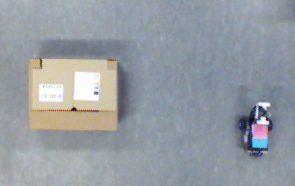
\includegraphics[width=\textwidth]{emptyGrid}
\caption{Forsøgsopstillingen inden hver test sættes i gang.}
\label{evaluering:emptyGrid}
\end{figure}
\subsection{Resultater}

\subsection{Opsummering}